\documentclass[14pt]{beamer}
\title[COJ:Java:05]{COJ :: Abstract Classes \& Interfaces}
\author[TS]{TalentSprint}
\institute[L\&D]{Licensed To Skill}
\date{Version 1.0.4}
\usefonttheme{serif}
\usecolortheme{orchid}
\usepackage{bookman}
\usepackage{hyperref}
\usepackage[T1]{fontenc}
\usepackage{graphicx}
\graphicspath{{../../Images/}}
\usepackage{listings}
\beamertemplateballitem
\usebackgroundtemplate{
\includegraphics[width=\paperwidth]{TS-Logo.jpg}}
\lstset{language=Java,numbers=left, numberstyle=\tiny, numbersep=10pt, showstringspaces=false, breaklines=true,keepspaces=true, columns=flexible}
\begin{document}

\begin{frame}
  \titlepage
\end{frame}

\begin{frame}{Learning Objectives}
The content in this presentation is aimed at teaching  learners to:
  \begin{itemize}
  \item Define abstract class
  \item Explain why abstract classes are needed
  \item Use abstract classes in writing small java applications
  \item Define interface
  \item Use interfaces in writing small java applications
  \item Use ``final'' keyword
  \end{itemize}
\end{frame}

\begin{frame}{Abstract Classes \& Interfaces}
Abstract class
 \begin{itemize}
  \item Is a conceptual class
  \item Provides a common root for a group of classes, nicely tied together in a package
  \item Cannot be instantiated -- objects cannot  be created
 \end{itemize}
\end{frame}

\begin{frame}[fragile]{Abstract Classes \& Interfaces}
 \begin{block}{Abstract class syntax}
  \begin{lstlisting}[numbers=none,  basicstyle=\tiny]
   abstract class ClassName {
       ...
       abstract Type MethodName1();
       ...
       Type Method2() {
           // method body
       }
   }
  \end{lstlisting}
 \end{block}
\begin{itemize}
 \item When a class contains zero or more abstract methods, it should be declared as abstract class
 \item The abstract methods of an abstract class must be defined in its subclass
 \item We cannot declare abstract constructors or abstract static methods
\end{itemize}
\end{frame}

\begin{frame}[fragile]{Abstract Classes \& Interfaces}
Abstract Class - Example
 
\includegraphics[scale=.4]{abstract-shape.png}
\begin{lstlisting}[numbers=none,  basicstyle=\tiny, frame=single, framexleftmargin=15pt]
public abstract class Shape {
    public abstract double area(); 
    public void move() { // non-abstract method
        // implementation
    }
}
 \end{lstlisting}
 Is the following statement valid?
 
 \fbox{\lstinline!Shape s = new Shape();!}
 
 No. It is illegal because the Shape class is an abstract class, which cannot be instantiated to create its objects
\end{frame}


\begin{frame}[fragile]{Abstract classes \& Interfaces}
 Abstract Classes
 \begin{lstlisting}[numbers=none,  basicstyle=\tiny]
public Circle extends Shape {
    protected double r;
    protected static final double PI = 3.1415926535;
    public Circle() {
        r = 1.0; 
    }
    public double area() { 
        return PI * r * r; 
    }
}

public Rectangle extends Shape {
    protected double w, h;
    public Rectangle() { 
        w = 0.0, h = 0.0; 
    } 
    public double area() {
        return w * h; 
    }
}
 \end{lstlisting}
\end{frame}

\begin{frame}[fragile]{Abstract Classes \& Interfaces}
Abstract Classes Properties

A class with one or more abstract methods is automatically abstract and it cannot be instantiated
\begin{lstlisting}[numbers=none,  basicstyle=\tiny, frame = single]
public abstract class Shape {
    public abstract double area(); 
    public void move() { // non-abstract method
        // implementation
    }
}
\end{lstlisting}
\lstinline!Shape s = new Shape(); // Error!
\end{frame}

\begin{frame}[fragile]{Abstract Classes \& Interfaces}
 \textbf{Abstract Classes Properties}
 
 A class declared abstract, even with no abstract methods can not be instantiated
 \begin{lstlisting}[numbers=none,  basicstyle=\tiny, frame = single]
public abstract class Triangle {
    private int radius;
    public double area() { // non-abstract method
        // implementation
    } 
    public void move() { // non-abstract method
        // implementation
    }
}
\end{lstlisting}
\lstinline!Triangle triagle = new Triangle(); // Error!
\end{frame}

\begin{frame}[fragile]{Abstract Classes \& Interfaces}
 \textbf{Abstract Classes Properties}
 
 A subclass of an abstract class can be instantiated if it overrides all abstract methods by implementation them
 \begin{lstlisting}[numbers=none,  basicstyle=\tiny, frame = single]
  public abstract class Shape {
    public abstract double area(); 
    public void move() { // non-abstract method
        // implementation
    }
}
public Rectangle extends Shape {
    protected double w, h;
    public Rectangle() { w = 0.0; h=0.0; }
    public double area() { return w * h; }
}
 \end{lstlisting}
\lstinline!Rectangle rectangle = new Rectangle(); // Legal!
\end{frame}


\begin{frame}[fragile]{Abstract Classes \& Interfaces}
 \textbf{Abstract Classes Properties}
 
 A subclass that does not implement all of the superclass abstract methods is itself abstract; and it cannot be instantiated
 \begin{lstlisting}[numbers=none,  basicstyle=\tiny, frame = single]
  public abstract class Shape {
    public abstract double area(); 
    public void move() { // non-abstract method
        // implementation
    }
}
public abstract Rectangle extends Shape {
    protected double w, h;
    public Rectangle() { w = 0.0; h=0.0; }
}
 \end{lstlisting}
\lstinline!Rectangle rectangle = new Rectangle(); // Illegal!
\end{frame}

\begin{frame}{Abstract Classes \& Interfaces}
 \textbf{Interfaces}
 \begin{itemize}
  \item Interface  is a  conceptual entity similar to an Abstract class
  \item Can contain only constants (final variables) and abstract method (no implementation) - Different from Abstract classes
  \item Use when a  number of classes share a common interface. Each class should implement the interface
 \end{itemize}
\end{frame}

\begin{frame}{Abstract Classes \& Interfaces}
 \texttt{Interfaces: An informal way of realising multiple inheritance}
 
 \begin{itemize}
  \item An interface is basically a kind of class - it contains methods and variables, but they have to be only abstract classes and final fields/variables
  \item Therefore, it is the responsibility of the class that implements an interface to supply the code for methods
  \item A class can implement any number of interfaces, but cannot extend more than one class at a time. Therefore, interfaces are considered as an informal way of realising multiple inheritance in Java
 \end{itemize}
\end{frame}

\begin{frame}{Abstract Classes \& Interfaces}
 \textbf{Interface - Example}
 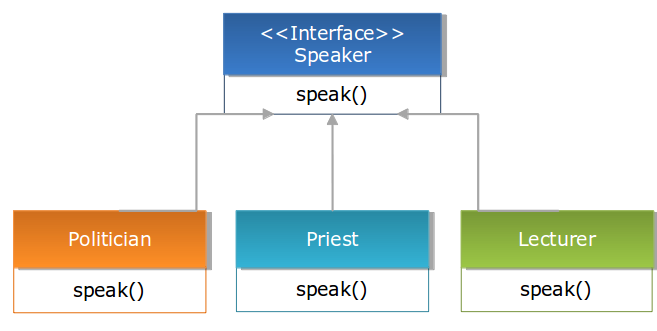
\includegraphics[scale=.45]{interface-example.png}
\end{frame}

\begin{frame}[fragile]{Abstract Classes \& Interfaces}

 \begin{block}{Interface Syntax}
  \begin{lstlisting}[numbers=none, basicstyle=\tiny]
interface InterfaceName {
    // Constant/Final Variable Declaration
    // Methods Declaration - only method body
}
  \end{lstlisting}

 \end{block}

 \begin{block}{Interface Example}
  \begin{lstlisting}[numbers=none]
interface Speaker {
    public void speak( );
}
  \end{lstlisting}

 \end{block}
\end{frame}

\begin{frame}[fragile]{Abstract Classes \& Interfaces}
 \textbf{Implementing Interfaces}
 
 Interfaces are used like super-classes who properties are inherited by classes. This is achieved by creating a class that implements the given interface as follows: 
 \begin{lstlisting}[numbers=none, frame = single]
class ClassName implements InterfaceName [InterfaceName1, InterfaceName2, ...] {
    // Body of Class
}
 \end{lstlisting}
\end{frame}

\begin{frame}[fragile]{Abstract Classes \& Interfaces}
\textbf{Implementing Interfaces Examples}
\begin{lstlisting}[numbers=none, frame = single, basicstyle=\tiny]
class Politician implements Speaker {
    public void speak() {
        System.out.println(``Talk politics'');
    }
}
\end{lstlisting}
\begin{lstlisting}[numbers=none, frame = single, basicstyle=\tiny]
class Priest implements Speaker {
    public void speak() {
        System.out.println(``Religious Talks'');
    }
}
\end{lstlisting}
\begin{lstlisting}[numbers=none, frame = single, basicstyle=\tiny]
class Lecturer implements Speaker {
    public void speak() {
        System.out.println(``Talks Object Oriented Design and Programming!'');
    }
}
\end{lstlisting}
\end{frame}

\begin{frame}[fragile]{Abstract Classes \& Interfaces}
 \textbf{Inheritance and Interface Implementation}
 \begin{block}{A general form of interface implementation:}
 \begin{lstlisting}[numbers=none, basicstyle=\tiny]
class ClassName extends SuperClass implements InterfaceName [, InterfaceName2, ...] {
    // Body of Class
}
\end{lstlisting}
\end{block}
This shows a class can extended another class while implementing one or more interfaces. It appears like a multiple inheritance (if we consider interfaces as special kind of classes with certain restrictions or special features)
\end{frame}

\begin{frame}{Abstract Classes \& Interfaces}
 \textbf{Final}
 \begin{figure}[H]
 \centering
 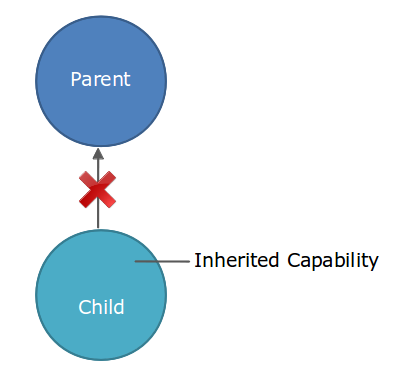
\includegraphics[scale=.4]{final.png}
 \end{figure}
\end{frame}

\begin{frame}[fragile]{Abstract Classes \& Interfaces}
 \texttt{Final Classes: A way for Preventing Classes being extended}
 
 We can prevent an inheritance of classes by other classes by declaring them as final classes. This is achieved in Java by using the following keyword final:
 \begin{lstlisting}[numbers=none, frame=single, basicstyle=\tiny]
final class Marks { 
    // members
}
final class Student extends Person { 
    // members
}
\end{lstlisting}
Any attempt to inherit these classes will cause an error.
\end{frame}

\begin{frame}{Abstract Classes \& Interfaces}
Final Members: A way for Preventing Overriding of Members in Subclasses
\begin{itemize}
 \item All methods and variables can be overridden by default in subclasses
 \item This can be prevented by declaring them as final using the keyword ``final'' as a modifier
 \item Example:
 
  \lstinline!final int marks = 100;!
  \lstinline!final void display();!
  \item This ensures that functionality defined in this method cannot be altered any. Similarly, the value of a final variable cannot be altered
 
\end{itemize}
\end{frame}

\begin{frame}{Abstract Classes \& Interfaces}
 \begin{figure}[H]
 \begin{center}
   
\includegraphics[scale=.3]{qa.png}   
 \end{center}
  \end{figure}
\end{frame}
\end{document}
